The PFA was implemented within the RISC-V ecosystem. RISC-V is an open-source instruction set with several open and closed-source implementations and ports for many common software components\cite{riscv}. I used the RISC-V port of Linux 4.13\cite{rvLinux} with a Buildroot generated user space\cite{rvBuildroot}.

\subsection{PFA Reference Implementation}
In order to accelerate software development, and to provide a golden-model of PFA behavior, I implemented the PFA first in a RISC-V ISA simulator called "Spike"\cite{spike}. Spike provides a functional simulation of a RISC-V core through a straightforward C++ interpreter, but does not provide any timing accuracy. Due to its simplicity, the PFA implementation required only a few weeks of implementation effort and less than 1000 LoC. With Spike, software development was able to proceed concurrently with the concrete hardware design.  Furthermore, unit tests developed under Spike were used to validate the hardware implementation, reducing debugging effort. In all, the only software change that was needed to go from Spike to a concrete implementation was one extra TLB flush due to a difference in TLB design between Spike and the RISC-V implementation we used.

\subsection{Concrete Implementation}
The PFA was implemented in the Chisel hardware construction language\cite{chisel} and integrated with a simple in-order CPU called RocketCore\cite{rocketCore}. The components were integrated using the RocketChip system-on-chip (SoC) generator\cite{rocketChip}. The hardware implementation of this system involved a large number of contributors and is not the main focus of this thesis\todo{How should I properly cite other contributors and make clear that this work was not done by me?}. I provide here an overview of a few relevant subsystems.

\subsubsection{RocketCore and RocketChip}
RocketChip is a framework for generating SoCs. It includes on-chip interconnects, caches, and other utilities for chip construction. While the CPU is pluggable, we use only the RocketCore in-order CPU for our experiments. Our implementation used dedicated 16KB instruction and data caches\todo{I hope to run experiments with an L2 in the future}. 

\subsubsection{PFA Implementations}

\subsection{Linux Integration} \label{sec_linuxImpl}
    We modified the Linux kernel (version 4.15\cite{linux}) to support the PFA. The
majority of software development was done using the functional simulator. Linux
is a mature open-source project with a long development history, resulting in
many Linux-specific terms. I will define these terms throughout this discussion
but you may refer to the glossary for a reference of terms.

\subsubsection{Non-PFA Paging in Linux} \label{sec:vanillaLinux}
I will now briefly describe how paging works in vanilla Linux. Note that the
kernel internally uses the term \gls{swap} in reference to all paging activity,
I will use these terms interchangeably. For a more complete discussion of
memory management in Linux, see \cite{linuxBook}. Figures
\ref{fig:vanilla_evict} and \ref{fig:vanilla_fetch} map out the steps involved
in evicting and fetching pages, respectively.

\paragraph{Page Reclaiming}
Linux manages memory limits on a per-task basis. In this case, a \gls{task}
refers to the kernel-specific abstraction of a process. Each task has its own
resource limits which are exposed to system administrators through the
\gls{cgroup} interface. When a task approaches its assigned limit of a certain
resource, it is throttled in a resource-specific manner. In the case of memory,
the kernel attempts to free task-assigned memory. It will first attempt to
shrink any file caches (especially clean disk blocks that can simply be deleted
without requiring any disk activity). If shrinking caches is not enough, the
kernel begins to page non-file backed pages (called ``\glspl{anonpg}''). This
is done using a pseudo-\gls{lru} eviction algorithm (Step 2 in Figure
\ref{fig:vanilla_evict}). Page reclaiming can be triggered
in one of two ways (Step 1). If a hard memory limit is met, but more memory is needed to
proceed, then page-reclaiming happens synchronously (called direct reclaim).
However, Linux tries to avoid this scenario by running a background thread
called \gls{kswapd} that begins reclaiming pages when the application reaches a
soft resource limit. \Gls{kswapd} is usually idle, but can be woken up when the
kernel detects a soft limit has been met. It also runs with a low priority to
avoid wasting resources on speculative evictions (the application may never hit
its hard limit).

\begin{figure}[h] \centering
  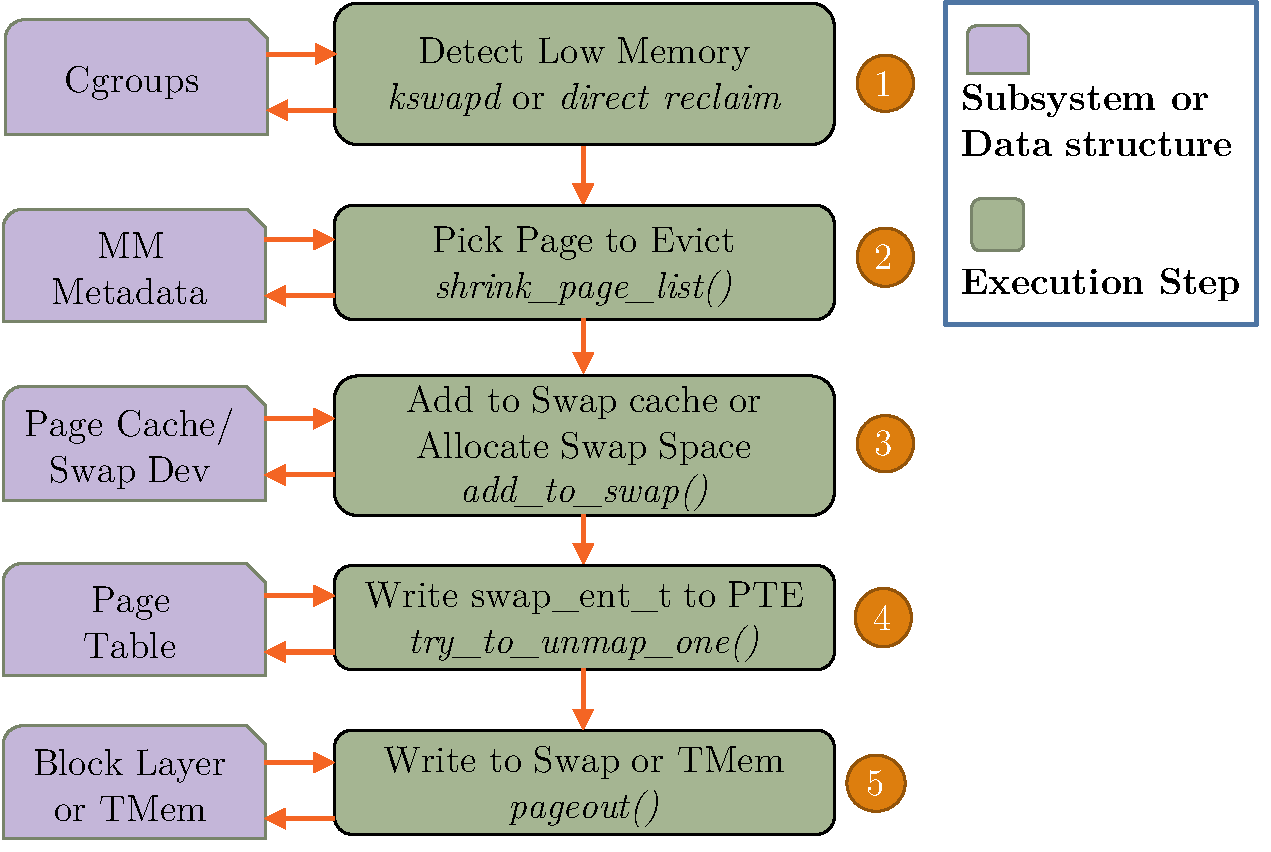
\includegraphics[width=0.7\textwidth]{vanilla_evict.pdf}
  \caption{Baseline Linux page eviction (reclaim) code path.}
  \label{fig:vanilla_evict}
\end{figure}

\paragraph{Page Eviction}
Paging was originally intended to use hard disks as backing store, and this is
reflected in the design of paging in Linux. To swap, one or more block
devices must be formatted and mounted as swap devices. Linux then uses the
block offset on this disk as a unique identifier for an evicted page (Step 3). In
order to support more complex paging schemes (such as page compression, or
heterogeneous memory), Linux introduced the \gls{tmem} layer\cite{tmem}. This
scheme still uses disk offsets as identifiers, but completely bypasses the block
layer. This is important because many optimizations in the block layer (e.g.,
write coalescing and block reordering) are not suitable for these alternative
paging devices. Evictions do not immediately result in writes to \gls{tmem} or
a swap device. Instead, pages are stored in a data structure called the swap
cache (Step 3). This swap cache helps reference count shared pages, and hedges
against poor eviction choices. Once a page is no longer physically available,
Linux replaces the corresponding \gls{pte} with a \gls{swpent} which clears the
valid bit, and uses the remaining bits to store the swap device ID (called
``type'' in the kernel) and block ID (called ``offset'') (Step 4).  When
changing a \glspl{pte}, most architectures require the OS to flush the
\gls{tlb}. This forces a page-table walk on the next access to this virtual
address. Finally, the kernel begins a write to the swap device in the
background (Step 5).

\paragraph{Page Fetch}

\begin{figure}[h] \centering
  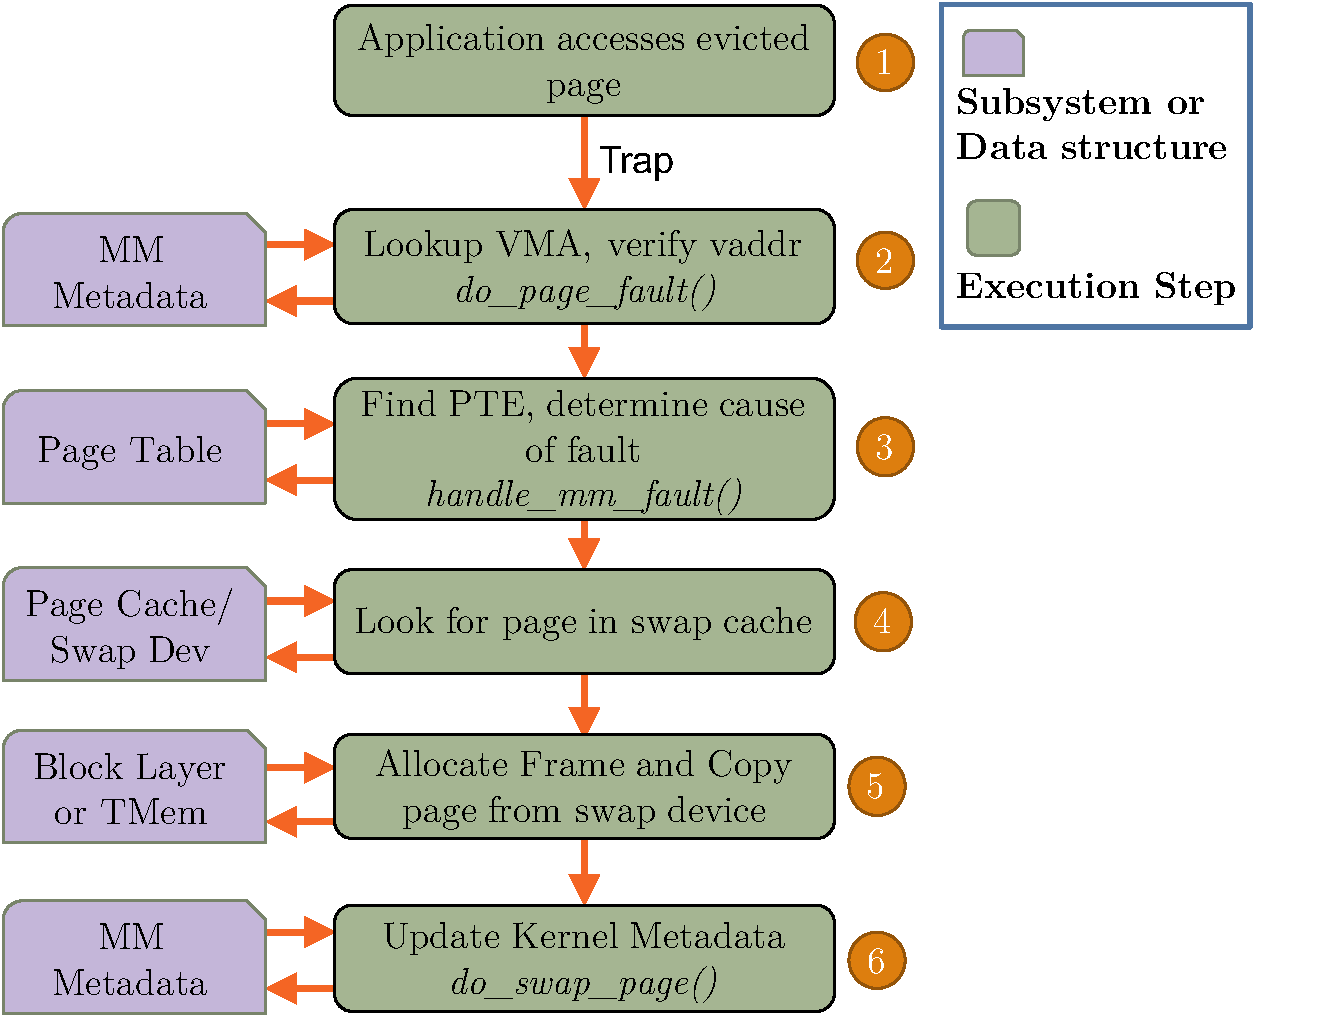
\includegraphics[width=0.7\textwidth]{vanilla_fetch.pdf}
  \caption{Baseline Linux page fetch code path.}
  \label{fig:vanilla_fetch}
\end{figure}

When a user program attempts to access a page that has been swapped out, the
\gls{ptw} notices the invalid PTE and issues a page fault trap to the OS (Step
1 in Figure \ref{fig:vanilla_fetch}). Note that the hardware does not examine
the remaining bits (the \gls{swpent} is purely a software construct). Upon
receiving a page fault, Linux first determines if the requested virtual address
has been assigned to this task. It does this by iterating through regions of
virtual memory called \glspl{vma} (Step 2). If a valid \gls{vma} is found, then
the OS begins a \gls{pgtbl} walk to locate the corresponding \gls{pte}. There
are several reasons that a page fault may occur, the OS must check the
\gls{pte} to determine the cause (Step 3). Assuming the cause was an invalid
\gls{pte}, the OS then searches the swap cache for this page (Step 4). This is
in case some other process that shares it has already brought it in. If the
page is not found, then a new frame is allocated and a transfer is initiated to
read the page from the swap device (Step 5). If the page is found in
\gls{tmem}, then the transfer occurs synchronously, otherwise the process
initiates the transfer and then yields to the scheduler, resulting in a context
switch. When the transfer is complete, the kernel changes the PTE from a
\gls{swpent} to a valid PTE with permissions defined by the \gls{vma}. Finally,
the kernel updates page-tracking meta-data (Step 6). This includes the \gls{lru} lists
maintained by the eviction algorithm, \gls{vma} membership, and a number of
other kernel subsystems. Note that several of these updates require
synchronization with other kernel threads. Once all bookkeeping is complete,
and the PTE is updated, the kernel flushes the \gls{tlb}, and restarts the
application.

\FloatBarrier 
\subsubsection{PFA Modifications}
The introduction of a PFA changes a number of the assumptions underlying
baseline paging behavior. Figure \ref{fig:linux_changes} summarizes these
changes.

\begin{figure}[h] \centering
  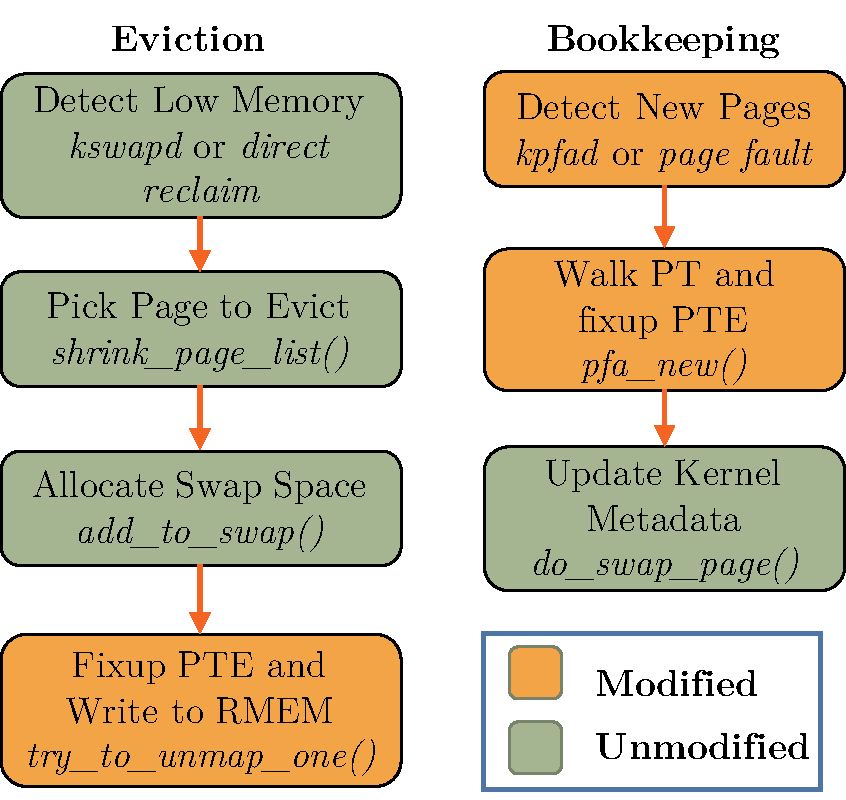
\includegraphics[width=0.5\textwidth]{linux_changes.pdf}
  \caption{Major changes to Linux paging to accommodate the PFA. Most
  subsystems could be re-used without change. On the eviction path, all that
  was changed was the PTE update (to write a remote \gls{pte} instead of a
  \gls{swpent}), and the write to disk (to write to remote memory instead). The
  bookkeeping path is now triggered either from the page-fault handler (due to
  a PFA service request) or from \gls{kpfad}. The core bookkeeping function
remains unmodified.}
  \label{fig:linux_changes}
\end{figure}

\paragraph{Frame Allocation and Permissions}
Linux uses the faulting virtual address to make a number of decisions during
the page fetch process. For instance, the permission bits are taken from the
\gls{vma}. \gls{vma} information is also used to decide which physical frame to
use (this is particularly important in NUMA systems). With the PFA, however,
the OS must decide on this information at \emph{eviction} time. Pre-allocating
physical frames is not an issue in our system because there is only one core,
and frame selection does not depend on the \gls{vma}. Permission bit selection
is more problematic. Our current approach is to assign permission bits to a
remote page based on the \gls{vma} permissions at the time of eviction, we then
update those permissions while performing bookkeeping. In practice, this is
unlikely to cause problems as permissions rarely change. Furthermore, Linux is
able to correct inappropriately restrictive permissions during page-faults.
However, there may be security concerns if permissions are made more
restrictive while a page is remote. This vulnerability exists in the window
between page fetch and bookkeeping. To mitigate this concern, the OS would need
to be modified to update remote PTEs when changing \gls{vma} permissions.

Under these simplifying assumptions, we are able to allocate frames
proactively. The current implementation always refills the \gls{freeq} during
bookkeeping. To simplify the bookkeeping procedure, we track
each allocated frame in a FIFO. This allows the bookkeeping code to simply pop
this FIFO to find which frame was used for each new page (the PFA always drains
the \gls{freeq} in FIFO order). Furthermore, this FIFO allows for aggressive
sanity checks that aided greatly in system debugging.

\paragraph{Asynchronous Bookkeeping}
In normal paging, the \emph{do\_swap\_page()} function is able to update meta-data as
soon as a page is fetched. With the PFA, we delay this bookkeeping for a
bounded but potentially non-trivial period of time. Many of these bookkeeping
tasks are in support of heuristics or resource accounting (e.g., LRU lists for
eviction, or memory utilization metrics). Delaying these tasks reduces the
accuracy of various algorithms, but does not result in incorrect behavior.
Others are needed for correct execution (e.g., \gls{vma} membership or shared
page tracking for copy-on-write). We address these correctness issues by
performing bookkeeping preemptively before accessing any of the related
algorithms. These tasks may be fairly common, but they are unlikely to actually
involve a recently fetched page. To avoid preemptively performing bookkeeping,
we use one of the reserved bits in the PTE protection field to indicate a page
that has been recently fetched but not yet processed. This bit gets set at
eviction time, but is cleared during bookkeeping.

\paragraph{Swap Device and Block ID Allocation}
Linux assumes that all swap activity is backed by a block device and it uses
the physical address on this device to identify all evicted pages. This block
ID is needed during the bookkeeping process to identify the page. To address
this problem we make a number of simplifying assumptions.

\begin{outline}[enumerate]
	\1 \textbf{A real swap device is available} (even though it is not used). We
		use a ram-based file system (ramfs) to trick the kernel into thinking it has
		a large disk attached. This uses no actual physical memory.
	\1 \textbf{There is only one swap device.} This allows us to not track device
		ID. This is achieved by making the ramfs sufficiently large to address all
		swap activity.
	\1 \textbf{Block IDs are contiguous on the integers $\mathbf{(0, 2^{28}]}$.}
		This allows us to pack the block ID into the remote PTE format (see Section
		\ref{sec:remPTE}). We achieve this by ensuring that the ramfs is the same
		size as our memory blade (and less than $2^{28}$ pages). Since block IDs
		correspond to physical offsets on the swap device, we are guaranteed to
		never see an invalid block ID.
\end{outline}

While these assumptions hold, we are able to compress the \gls{swpent} into a
\SI{28}{\bit} PageID by eliding the type, and using the offset directly.
Finally, we avoid overheads in the block layer by implementing the PFA as a
\gls{tmem} device. Since bookkeeping is asynchronous, and eviction occurs
earlier in the process (due to ordering constraints with PTE modifications),
this \gls{tmem} plugin simply returns immediately. The current implementation
evicts synchronously. This is because the expected write time is much smaller
than a scheduling quantum and asynchronous eviction would result in wasteful
context switches. Future implementations may attempt to overlap eviction with
low-latency tasks such as bookkeeping.

\subsubsection{kpfad} \label{sec:kpfad}
The most basic implementation of PFA support in Linux simply performs
bookkeeping tasks whenever the internal queues of the PFA fill up. This
effectively batches page bookkeeping, but it does not allow the kernel to
choose when the bookkeeping occurs. To leverage idle periods in
program execution, or unused hardware threads, we implement a background
bookkeeping daemon called \gls{kpfad}. \Gls{kpfad} is triggered by an adaptive
timer that attempts to discover the average time between full queues. It does
this by increasing the wait time by a small amount every time it runs, and
decreasing the time whenever the application is interrupted due to full queues. 
While \gls{kpfad} gives increased flexibility and efficiency on a lightly
loaded system, it causes strictly more overhead than interrupt-driven
bookkeeping when the application has enough work to keep all hardware threads
busy (since the adaptive timer is not perfect). To avoid this, \gls{kpfad} is run
with very low priority (similar to the page-out daemon \gls{kswapd}). Unlike
\gls{kswapd}, however, \gls{kpfad} does not get triggered by a soft limit. We expect
the adaptive timer scheme, coupled with low priority, to be sufficient to avoid
significant overhead.

\subsubsection{Baseline Swapping}
We modified Linux to use the remote memory blade while paging. This was done by
implementing a software interface to the remote memory blade as a \gls{tmem}
device. The swapping mechanism uses a custom NIC driver that provides zero-copy
semantics and bypasses the normal Linux networking stack. 

